\section{TRAJECTORY GENERATION}\label{method}

In table tennis, one needs to specify when, where and how to intercept the incoming ball trajectory $\ball(t)$. So far, most of the algorithms for robotic table tennis \cite{Matsushima05}, \cite{Muelling13} calculate the intersection point of an estimated ball trajectory $\ballEst(t)$ with a virtual hitting plane $z = z_{\mathrm{VHP}}$ to determine the space and time coordinates of the hitting point. It is possible to eliminate this plane altogether and include the striking time as another parameter to be determined in an optimization problem.

\subsection{Optimal Control for Trajectory Generation}

When generating striking trajectories for the robot, trajectories with minimal acceleration or jerk can be preferred for safety and efficiency reasons. We therefore consider the following \emph{free-time} optimal control problem~\cite{Liberzon11}
%
\begin{align}
&\min_{\ddot{\joint},T} \int\limits_{0}^{T}\ddot{\joint}(t)^{\mathrm{T}}\vec{R}\ddot{\joint}(t), \label{costFnc1} \\
\textrm{s.t. \ } & \kin(\joint(T)) = [\normal_{\mathrm{des}}(t),\ballEst(t)], \label{transCond1}\\
&\jac(\joint(T))\dot{\joint}(T) = \racketVel_{\mathrm{des}}(t), \label{transCond2} \\
&\joint(0) = \joint_{0}, \label{initCond1} \\
&\dot{\joint}(0) = \dot{\joint}_{0}, \label{initCond2}
\end{align}
%
\noindent where the final time $T$ of the racket trajectory is an additional variable to be optimized along with the joint accelerations $\ddot{\joint}(t) \in \mathbb{R}^{n}$. The direct kinematics function $\kin(\cdot)  \in \mathbb{R}^{3 \times 2}$ is the relevant submatrix of the homogeneous transformation $\vec{T}(\cdot) \in \mathbb{R}^{4 \times 4}$ giving the desired racket normal and racket center position at striking time. The sub-Jacobian $\jac(\joint(T)) \in \mathbb{R}^{3 \times n}$ gives the condition for the desired Cartesian racket velocities. $\vec{R} \succeq 0 \in \mathbb{R}^{n \times n}$ is a positive definite weighting matrix for the accelerations. Initial conditions for the robot are the joint positions $\joint_0$ and joint velocities $\dot{\joint}_0$.

Solution of \eqref{costFnc1} using Pontryagin's maximum principle is well known in the optimal control literature: the solution $\joint(t)$ is a third degree polynomial for each degree of freedom, with the \emph{transversality conditions} \eqref{transCond1} - \eqref{transCond2} imposing another condition on the Hamiltonian to satisfy at striking time~\cite{Schaettler12}. See Figure~\ref{mainIdea} for an illustration. % which figure 

In the above case with only boundary equality constraints, the striking time $T$ and the joint position and velocity values at striking time $\joint_f$ and $\dot{\joint}_f$ fully parametrize the polynomial and can be determined by solving a $2n+1$ dimensional equation~\footnote{For example using $\mathtt{fsolve}$ in MATLAB.}. Inspired by the simplicity of this solution, we extend the same parametrization to the constrained optimization, with joint position, velocity and acceleration limits imposed throughout the whole trajectory.

\begin{figure}[t!]
\centering
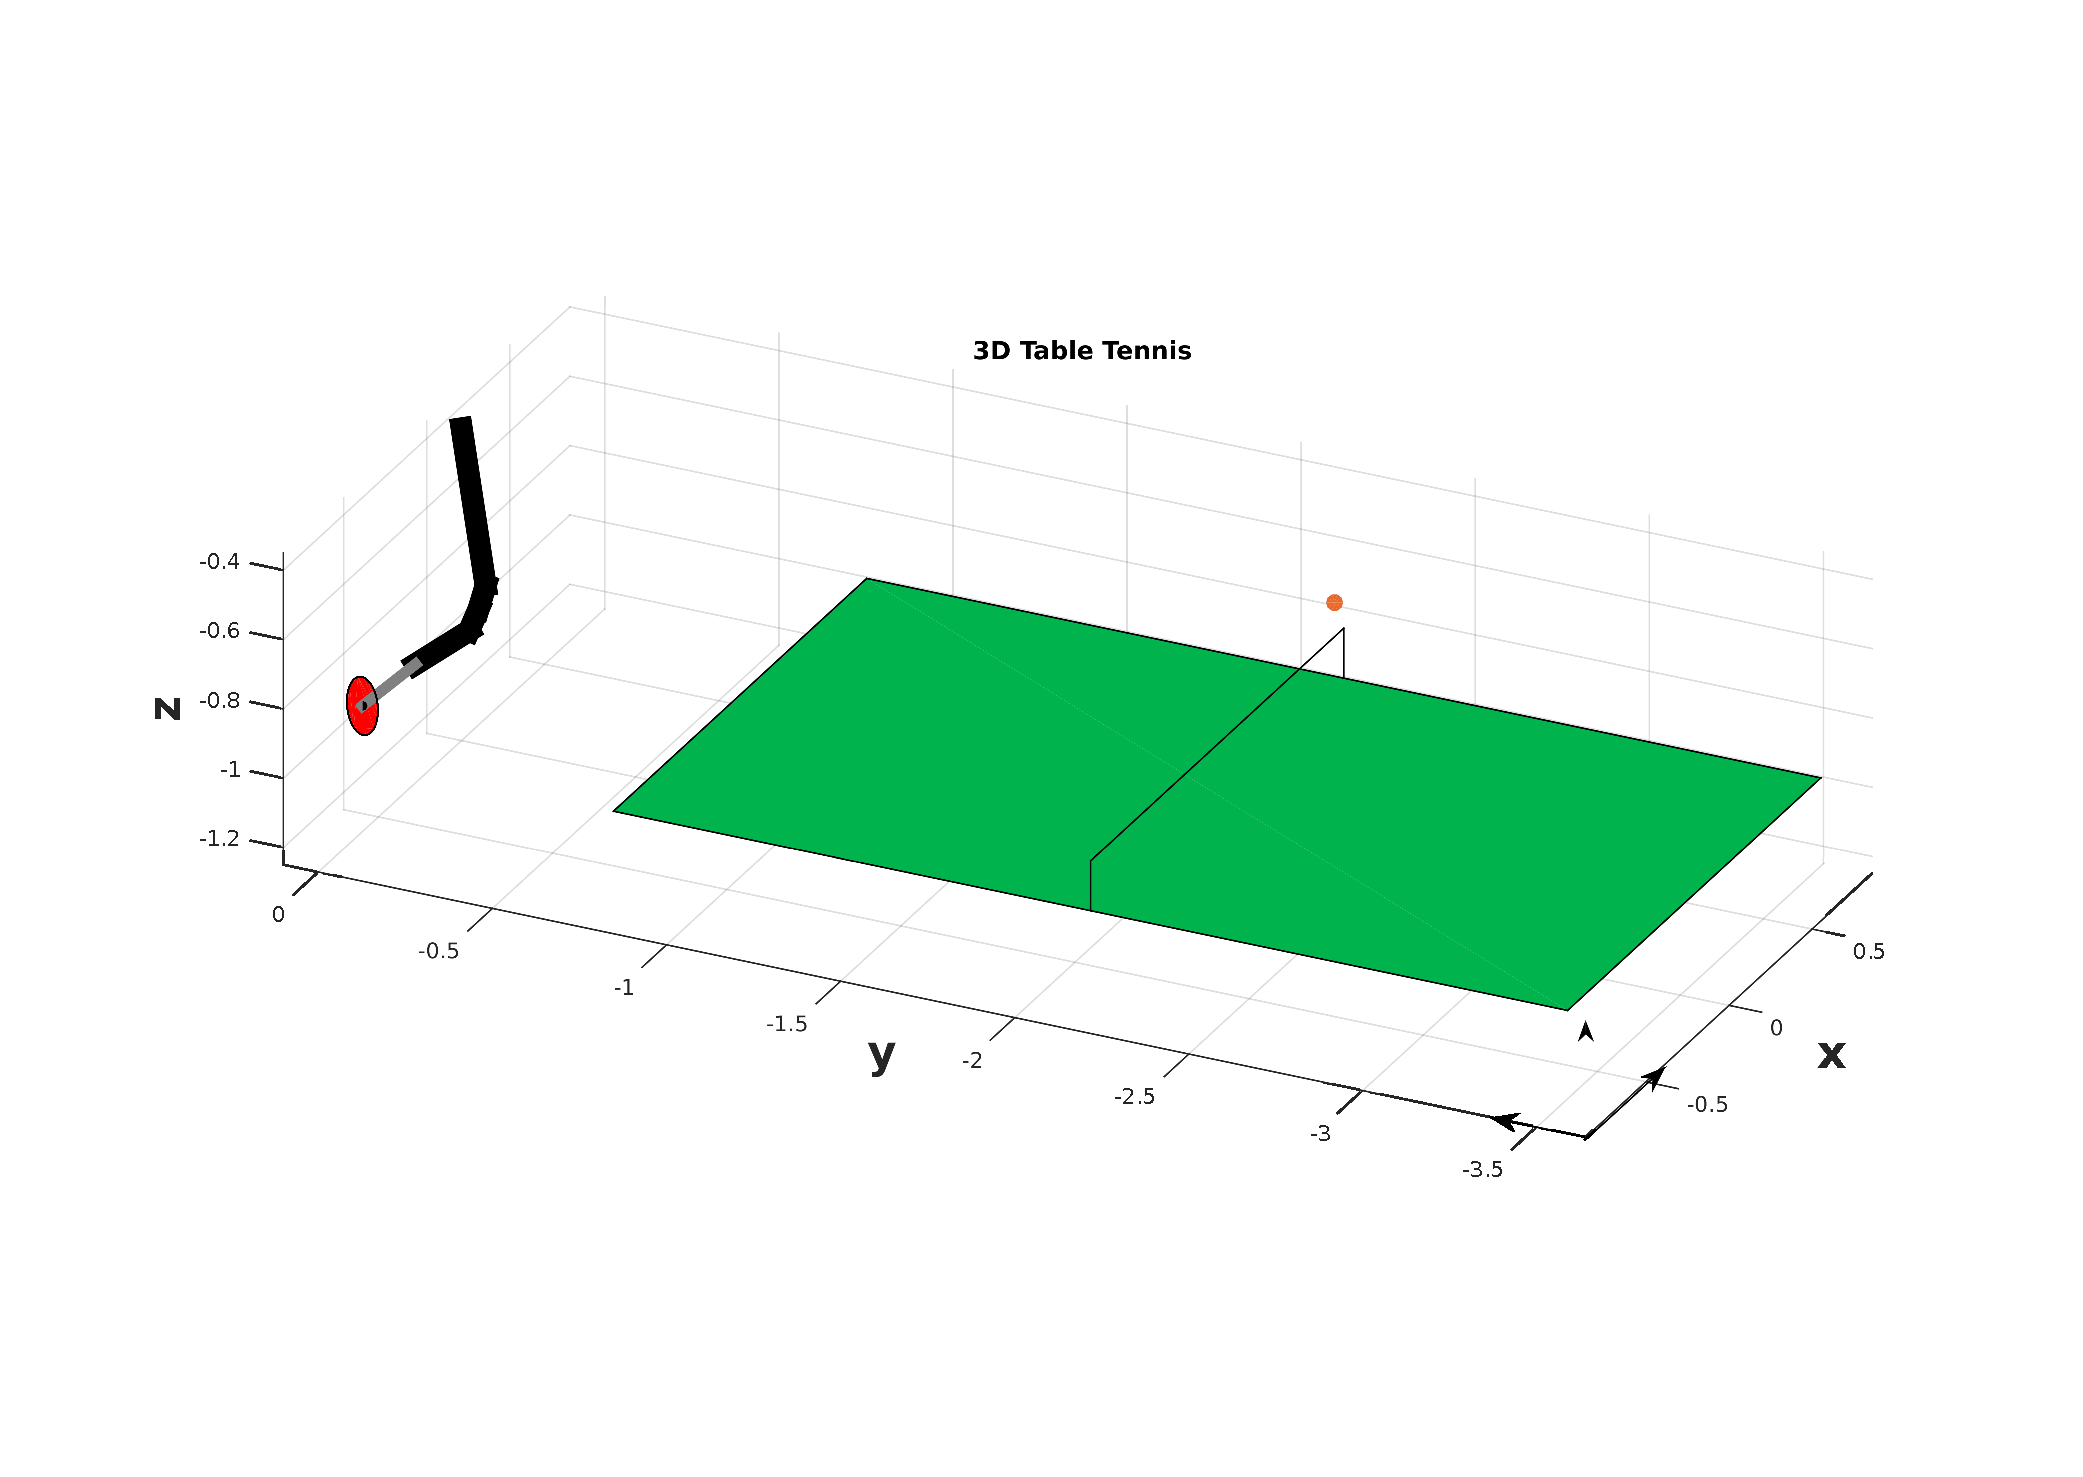
\includegraphics[scale=0.25]{tableTennis3D.eps}			
\caption{A schema for a three dimensional table tennis model. Ball is shown as an orange blob and the racket, in resting state, is shown in red. We predict the path of the ball using models that we train from actual data: the ballistic flight model, the rebound model and the racket-ball landing model respectively. The trajectory generation framework takes as input a desired racket trajectory calculated using these models.}
\label{models}
\end{figure}

\subsection{Predicting with Probabilistic Modeling}\label{sectionPredict}
 
In this framework, we require three models to determine the equality constraints~\eqref{transCond1} - \eqref{transCond2} for the trajectory generation process. We first need to predict the future ball trajectory $\ballEst(t)$ from noisy ball observations.  The ballistic \emph{flight model} is a nonlinear model $\ddot{\ball} = \ballDynamics(\dot{\ball})$ that describes the dynamics of the ball $\ball = (b_x,b_y,b_z)^{\mathrm{T}}$. It involves air drag $\drag$ and gravity $\gravity$
%
\begin{align}
\begin{bmatrix}
   \ddot{b_x} \\
   \ddot{b_y} \\
   \ddot{b_z}   
 \end{bmatrix} &= 
 \begin{bmatrix}
 -\drag \ballVel \dot{b}_x  \\
 -\drag \ballVel \dot{b}_y  \\
 \ \gravity - \drag \ballVel \dot{b}_z 
 \end{bmatrix},
\label{flightModel}
\end{align}
%
\noindent where $\ballVel = \|\dot{\ball}\|_2$ is the velocity of the ball. We use a linear model for the \emph{rebound model}
%
\begin{align}
\dot{\ball}_{\mathrm{out}} = \bounce\dot{\ball}_{\mathrm{in}}.
\label{reboundModel}
\end{align}

\noindent The rebound model \eqref{reboundModel} is a discrete event which reflects the ball when the ball is touching the table. Matrix $\bounce$ in \eqref{reboundModel} is a diagonal matrix with entries $\vec{\epsilon} = [\epsilon_{x}, \epsilon_{y}, -\epsilon_{z}]^{\mathrm{T}}$. The coefficient of restitution $\epsilon_{z} \in (0,1)$ accounts for the reflection of velocity in the vertical direction $z$ and $\epsilon_{x}, \epsilon_{y} \in (0,1)$ are the coefficients of friction along the planar $x,y$ directions. See Figure~\ref{models} for a table tennis schema. 

The accuracy of the rebound model~\eqref{reboundModel} clearly depends on that of the flight model~\eqref{flightModel}, so we first train the parameters of the flight model using nonlinear least squares. Secondly, we use the trained flight model to smoothen the ball path before rebound and after rebound. Using an Extended Kalman Smoother, we can calculate the ball velocities before and after rebound and then use linear least squares to estimate the rebound parameters. A more comprehensive approach would be to train the two models together with a smoothing Expectation-Maximization (EM) algorithm, at no apparent advantage. % cite needed
Effects of ball angular velocity, or in other words spin, are not accounted for in these models.

During test time we use the same trained Extended Kalman Filter (EKF) to perform prediction on the filtered ball state. Any other regression method to estimate initial ball position and velocity can also be used. Using an EKF for our nonlinear model \eqref{flightModel} generates at each time instant $t$ a probability distribution $p_t(\ball,\dot{\ball}|t)$ of incoming ball states parameterized by time, 
%
\begin{align}
\ball(t) &\sim \mathcal{N}(\vec{\mu}_{\textrm{in}}(t),\vec{\Sigma}_{\textrm{in}}(t)). 
\label{ballProcess}
\end{align}

